%!TEX output_directory = tmp
\documentclass[11pt, aspectratio=169]{beamer}
\usepackage[utf8]{inputenc}
\usepackage[russian]{babel}
\usepackage{subcaption}
\usepackage{ITMOtemplate}


\newcommand{\R}{\mathbb{R}}
\pdfstringdefDisableCommands{\let\uppercase\@firstofone}

\graphicspath{{figs/}}

\newcommand{\Code}[1]{\textbf{#1}}
\newcommand{\bb}[1]{\mathbb{#1}}
\newcommand{\cc}[1]{\mathcal{#1}}

\title{\centering Исследование методов кинодинамического\\ планирования движения роботов}

\author[Author, Another]{
    \hfill
    {\bf Антипов В.А.}\inst{1}
    \hfill
}

\institute[ITMO University] % (optional, but mostly needed)
{
    \hfill
    \begin{minipage}[t]{0.4\textwidth}
        \centering{\inst{1}%
        ITMO University}
    \end{minipage}
    \hfill
 }

\date[Occasion]{\today \\ Пятидесятая научная и учебно-методическая конференция Университета ИТМО}

\begin{document}

\frame{\titlepage}

\section{Введение}
% 
\begin{frame}{Актуальность}
    \begin{figure}[ht]
        \begin{subfigure}[b]{0.48\textwidth}
             \centering
             \includegraphics[width=0.9\textwidth]{figures/part1.JPG}
             \caption{База}
             \label{fig:rozum}
         \end{subfigure}
         \hfill
         \begin{subfigure}[b]{0.48\textwidth}
             \centering
             \includegraphics[width=0.9\textwidth]{figures/part3.JPG}
             \caption{Звено}
             \label{fig:ur}
         \end{subfigure}
         \hfill
         \begin{subfigure}[b]{0.48\textwidth}
             \centering
             \includegraphics[width=0.9\textwidth]{figures/part4.JPG}
             \caption{Крепления}
             \label{fig:xarm}
         \end{subfigure}
         \hfill
         \begin{subfigure}[b]{0.48\textwidth}
             \centering
             \includegraphics[width=0.9\textwidth]{figures/part5.JPG}
             \caption{Двигатели}
             \label{fig:xarm}
         \end{subfigure}
         \caption{Составные части модуля}
    \end{figure}

\end{frame}

% \begin{frame}{Модульный подход}
    
%     \begin{figure}[ht]
%         \begin{subfigure}[b]{0.3\textwidth}
%          \centering
%          \includegraphics[width=0.7\textwidth]{figures/mod1.png}
%          \caption{Rozum}
%          \label{fig:rozum}
%      \end{subfigure}
%      \hfill
%      \begin{subfigure}[b]{0.3\textwidth}
%          \centering
%          \includegraphics[width=0.9\textwidth]{figures/mod2.png}
%          \caption{UR5}
%          \label{fig:ur}
%      \end{subfigure}
%      \hfill
%      \begin{subfigure}[b]{0.3\textwidth}
%          \centering
%          \includegraphics[width=0.7\textwidth]{figures/mod3.png}
%          \caption{Xarm}
%          \label{fig:xarm}
%      \end{subfigure}
%      \caption{Модульные коллаборативные роботы}
%     \end{figure}
% \end{frame}

% \begin{frame}{Проектирование модуля}
%     \begin{figure}[ht]
%         \begin{subfigure}[b]{0.48\textwidth}
%          \centering
%          \includegraphics[width=0.9\textwidth]{figures/part1.JPG}
%          \caption{База}
%          \label{fig:rozum}
%      \end{subfigure}
%      \hfill
%      \begin{subfigure}[b]{0.48\textwidth}
%          \centering
%          \includegraphics[width=0.9\textwidth]{figures/part3.JPG}
%          \caption{Звено}
%          \label{fig:ur}
%      \end{subfigure}
%      \hfill
%      \begin{subfigure}[b]{0.48\textwidth}
%          \centering
%          \includegraphics[width=0.9\textwidth]{figures/part4.JPG}
%          \caption{Крепления}
%          \label{fig:xarm}
%      \end{subfigure}
%      \hfill
%      \begin{subfigure}[b]{0.48\textwidth}
%          \centering
%          \includegraphics[width=0.9\textwidth]{figures/part5.JPG}
%          \caption{Двигатели}
%          \label{fig:xarm}
%      \end{subfigure}
%      \caption{Составные части модуля}
%     \end{figure}
% \end{frame}


% \section{Модель обучения}

% \begin{frame}{Математическая модель модульногодизайна робота}
%     \begin{columns}[onlytextwidth]
%         \begin{column}{0.45\textwidth}
%             \begin{itemize}
%               \item $t = 0,1,2,\dots$ -- дискретные промежутки времени,
%               \item $\cc{S}$ -- пространство состояний (Конфигурация дизайна),
%               \item $\cc{A}$ -- пространство действий (Какой модуль добавить),
%               \item $R_t = R(s_t, a_t): \cc{S}\times \cc{A} \rightarrow \bb{R}$ -- функция награды  агента за совершение действия $a_t$ из состояния $s_t$.
%             \end{itemize}
%         \end{column}
%         \begin{column}{0.5\textwidth}
%             \begin{figure}
%                 \centering
%                 \includegraphics[width=\textwidth]{figures/ref.png}
%                 \caption{Задача модульной сборки}
%                 \label{fig:my_label}
%             \end{figure}
%         \end{column}
%     \end{columns}
% \end{frame}

% \subsection{Математическая модель мультиагентной системы}

% \begin{frame}{Математическая модель мультиагентной системы}
%     \begin{columns}[onlytextwidth]
%         \begin{column}{0.65\textwidth}
%             \begin{itemize}
%               \item $t = 0,1,2,\dots$ -- дискретные промежутки времени,
%               \item $i = 0,1$ -- номер агента,
%               \item $\cc{S}$ -- пространство состояний агентов,
%               \item $\cc{A}^i$ -- пространство действий для $i$-го агента, $A = A_1 \times \dots \times A_N$,
%               \item $\cc{T}(s_t, a_t, s_{t+1}): \cc{S}\times \cc{A} \rightarrow \bb{P}(s_{t+1} | s_t, a_t)$ -- функция совершения из совместного состояния $s_t$ совместного действия $a_t=(a_t^1,a_t^2, \dots)$ и принятия совместного состояния $s_{t+1}$,
%               \item $R^i_t = R(s_t, a^i_t): \cc{S}\times \cc{A}^i \rightarrow \bb{R}$ -- индивидуальная функция награды $i$-го агента за совершение действия $a^i_t$ из совместного состояния $s_t$.
%             \end{itemize}
%         \end{column}
%         \begin{column}{0.35\textwidth}
%             \begin{figure}
%                 \centering
%                 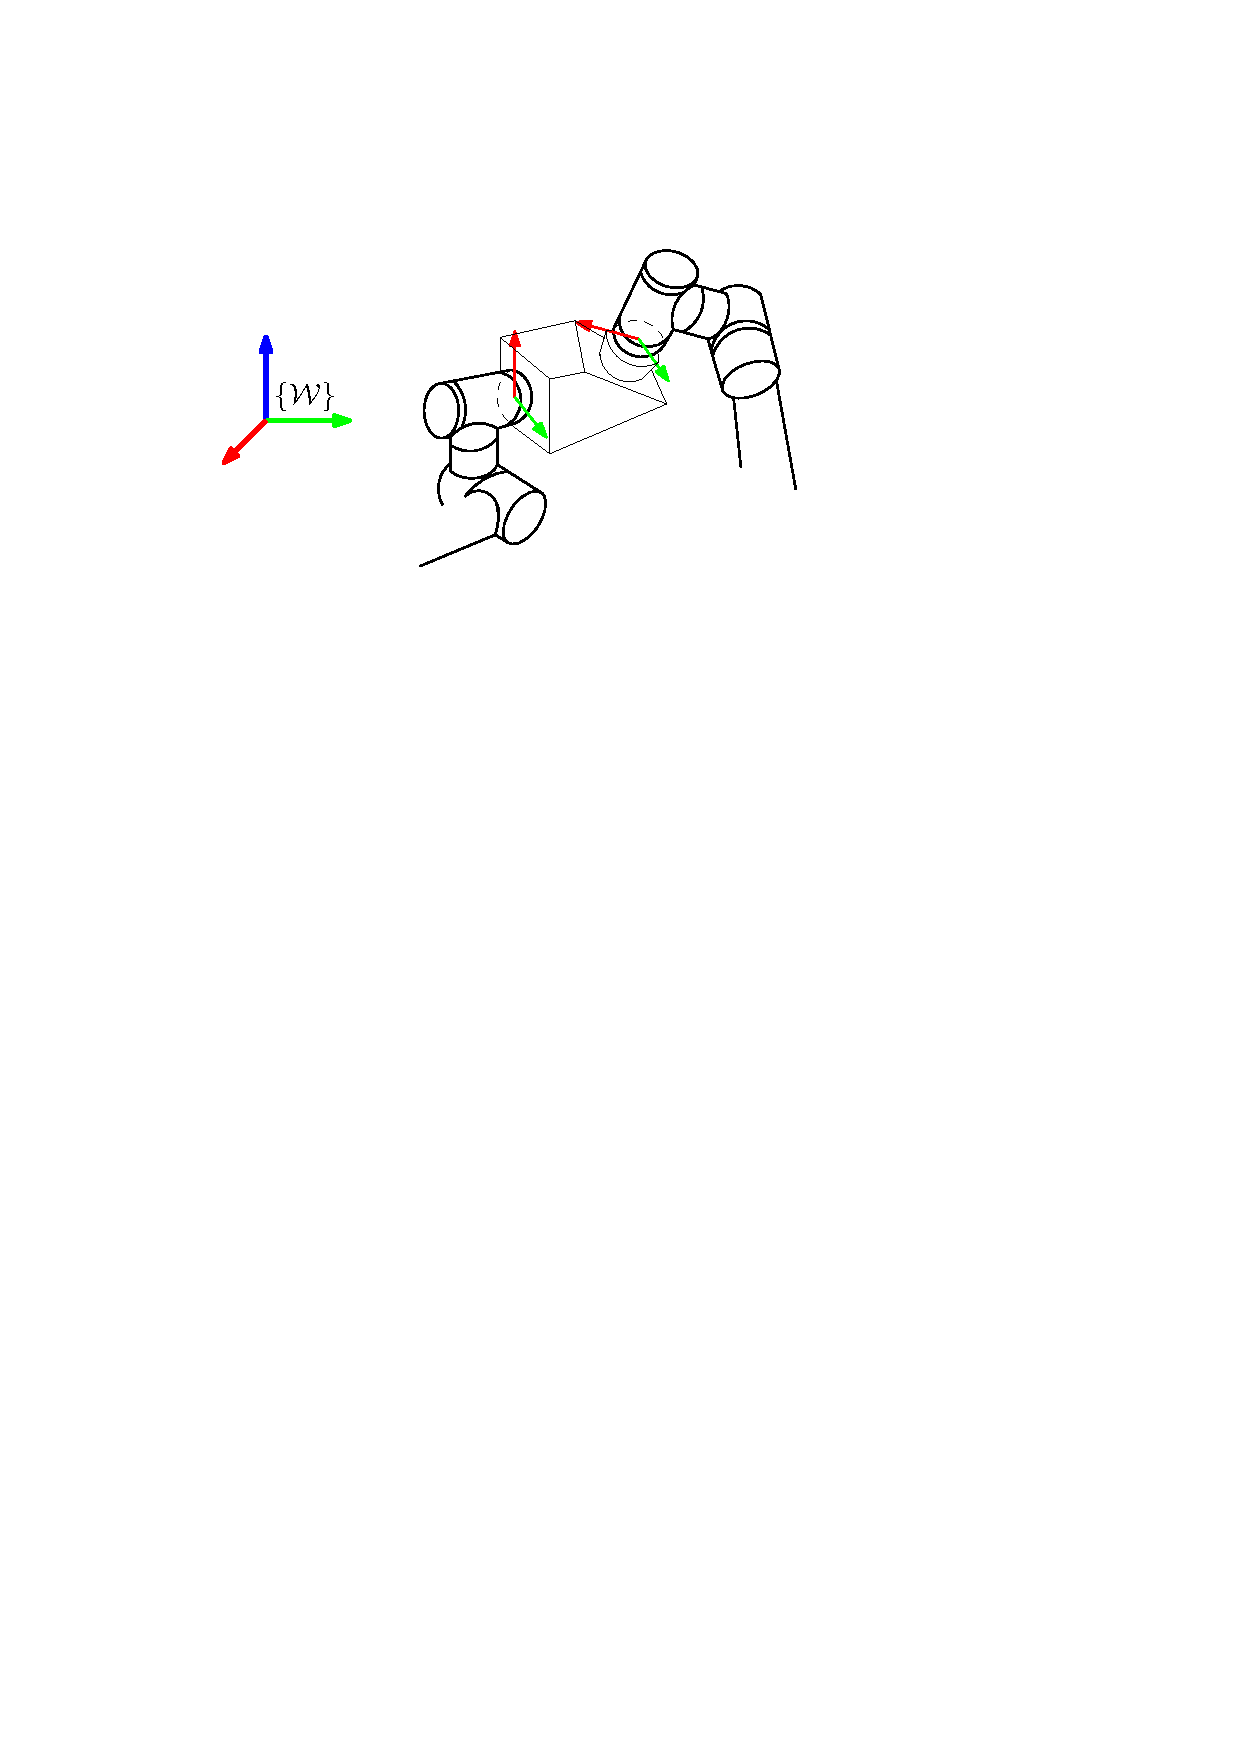
\includegraphics[width=\textwidth]{figures/object_coop_peginhole.pdf}
%                 \caption{Задача сборки деталей}
%                 \label{fig:my_label}
%             \end{figure}
%         \end{column}
%     \end{columns}
% \end{frame}

% \section{Цель обучения}

% \begin{frame}{Обучение агентов}
%     Целью каждого агента является максимизация индивидуального будущего выйгрыша  $G^i_{t}$. Для построения закона оптимального управления рассмотрим функцию полезности состояния-действия:
%     \begin{align}
%         \nonumber Q^{\pi_i}(s_t, a^i_t) = \bb{E}_{\pi_i}\left[ G^i_{t} | s_t, a^i_t \right] = \bb{E}_{\pi_i}\left[ \sum_k^\infty \gamma^t R^i_{t+k+1} | s_t, a^i_t \right] \\
%         = R^i_{t+1} + \gamma \bb{E}_{\pi_i}\left[G^i_{t+1}| s_t, a_t^i \right]
%     \end{align}
%     Необходимо найти такое оптимальное управление $\pi_i(s_t)$, что значение функции полезности состояния-действия принимает максимальное значение:
%     \begin{equation}
%         Q^{*\pi_i}(s_t, a^i_t) = R^i_{t+1} + \gamma \max_{\pi_i}  Q^{*\pi_i}(s_{t+1}, a^i_{t+1})
%     \end{equation}
% \end{frame}



\begin{frame}{Параметры разработанной среды}
    \begin{columns}[onlytextwidth]
        \begin{column}{0.59\textwidth}
            % \begin{figure}
            %     \centering
            %     \includegraphics[width=1.0\textwidth]{figures/rldesign.png}
            %     \caption{TinyBot}
            %     \label{fig:tinybot}
            % \end{figure}
        \end{column}
        \begin{column}{0.4\textwidth}
            Особенности разработанной среды:
            \begin{itemize}
                \item Пространство действий $A$ - дискретное
                \item Пространство состояний $S$ - векторное, дискретное
                \item Возможность гибкого выбора критерия оптимизации дизайна.
            \end{itemize}
        \end{column}
    \end{columns}
\end{frame}

\begin{frame}{Дальнейшая работа}
    \begin{columns}[onlytextwidth]
        \begin{column}{0.48\textwidth}
    
            % \begin{figure}
            %     \centering
            %     \includegraphics[width=0.7\textwidth]{figures/tinybot.png}
            %     \caption{TinyBot}
            %     \label{fig:tinybot}
            % \end{figure}
        \end{column}
        \begin{column}{0.5\textwidth}
            :
            \begin{itemize}
                \item Поиск оптимального дизайна разрабатываемого робота TinyBot
                \item Добавление в среду возможности более тонкого конфигурирования модулей
                \item Добавление моделирования динамики в среду
            \end{itemize}
        \end{column}
    \end{columns}
\end{frame}

\end{document}
